\chapter{Evaluation}
\label{ch: Verifikation}
Zur Evaluation der künstlichen neuronalen Netze wird eine anwendungsorientierte \textit{Benchmark} durchgeführt. Hierbei wird anhand der in Abschnitt \ref{subsec: Entwickeltes neuronales Netz} beschriebenen Datensätze die \textit{Precision-Recall}-Methode angewendet. Weiterhin werden die Benchmarks auf dem integrierten Computer des ALFs und einem eingebetteten System ausgeführt. Als eingebettetes System wird ein \textit{Raspberry Pi 3 Model B} verwendet. Die Eckdaten des integrierten Computers sind in der Masterthesis von M.Sc. \textit{Dominik Eickmann} und M.Sc. \textit{Dennis Hotze} dargestellt \cite{alf}. Es ist keine geräteübergreifende Veränderung der Genauigkeit je Netz zu erwarten, da die Eingangsdaten und die Rechenoperationen identisch sind. Jedoch können so die Bearbeitungszeiten pro Bild für unterschiedliche Hardwareplattformen verglichen werden. Eine präzise Auflistung aller gemessenen Analysezeiten ist in Tabelle \ref{fig: zeitentab} präsentiert. \\

Insgesamt werden für den Test 12755 Bilder von Personen aus dem Trainingsdatensatz entnommen. Der technische Hintergrund hierfür ist in Abschnitt \ref{subsec: Entwickeltes neuronales Netz} zu finden. Die Unterteilung des Datensatzes in Trainings- und Testdaten geschah vor dem Training. Andernfalls würde ein Netz während des Trainings mit bereits bekannten Eingangsdaten rechnen. Dies würde das Testergebnis verfälschen. Als Vergleich analysiert jedes Netz auch den eigenen Datensatz. So kann die Performance am Einsatzort des ALFs an der Hochschule Bochum evaluiert werden. Jedes Bild wird für die verwendeten, neuronalen Netze auf eine Pixelgröße von $300 \times 300$ skaliert. Für die Evaluation des \textit{HOG-SVM}-Systems wird eine höhere Auflösung gewählt. Hierbei wird eine Seite des Bildes softwareseitig auf 400 Pixel begrenzt. \\

Der im Grundlagenabschnitt \ref{subsec: evaluation neuronaler netze} beschriebene \textit{mAP}-Wert wird häufig auf Objekterkennungssystemen mit multiplen Klassen angewendet. Die hier entwickelte Personenerkennung soll jedoch lediglich die Klasse \textit{Person} erkennen. Somit ist der \textit{mAP}-Wert in diesem Fall der Mittelwert eines Messwerts und kann als Integral der \textit{Precision-Recall}-Kurve angesehen werden. Im Verlauf der Evaluation der angewendeten Systeme wird mithilfe einer Berechnungssoftware jeweils der \textit{mAP}-Wert berechnet.
 

\begin{figure}[H]
	\centering
	\begin{tikzpicture}[
	]
	\begin{axis}[
	width=12cm,
	height=7cm,
	axis y line*=left,
	ticklabel style={% gilt für x und y
		/pgf/number format/.cd,
		use comma,% Komma als Dezimaltrenner
		1000 sep = {}% keine Tausendertrennung 
	},
	xlabel={$\text{Recall } \textit{r(t)}$},
	ylabel={$\text{Precision } \textit{p(t)}$},
	axis x line*=bottom,
	xmin=0, xmax=0.3, 
	ymin=0, ymax=0.3,
	%every axis plot/.append style={line width=1.0pt}
	legend pos=north east,
	]
	
	\addlegendentry{Eigener Datensatz}; % legende1
	\addplot[gray, line width=0.8pt]  table [x=Step,y=Value,col sep=comma] from {Bilder/hog.csv};
	\addplot[black, line width=0.8pt]  table [x=Step,y=Value,col sep=comma] from {Bilder/hogcoco.csv};
	\addlegendimage{/pgfplots/refstyle=plotbrr};				
	\addlegendentry{\textit{COCO}-Datensatz} ;%legende 2;
	%\addlegendentry{plot 1}
	\end{axis}
	\end{tikzpicture}
	\caption{\textit{Precision-Recall}-Kurven des \textit{SSD MobileNet V2} Netz. Die schwarze Kurve beschreibt die Analyse durch den \textit{COCO}-Datensatz. Der Test mithilfe des eigenen Datensatz wir durch die graue Kurve präsentiert. https://github.com/kaka-lin/object-detection}
	\label{fig: ssdmobilenetv2}
\end{figure}


Die Kombination aus \textit{HOG} und \textit{SVM} erreicht in der Benchmark die in Abbildung \ref{fig: hog1} präsentierten Ergebnisse. Der \textit{mAP}-Wert liegt für den eigenen Datensatz bei 0,16 und für den \textit{COCO}-Datensatz bei 0,07. Die eingetragenen Begrenzungsrahmen stechen bei der Durchsicht der Ergebnisse durch ihren verhältnismäßig großen Umfang heraus. Dies lässt sich auf die Dimension der Zellen zurückführen. Eine Reduktion der Zellengröße könnte wiederum die Erkennung weiter verschlechtern. Der \textit{IoU}-Wert ist hierdurch entsprechend niedrig und führt zu diesem Ergebnis. Mit den entsprechende Optimierungen wurden die \textit{Precision-Recall} Werte für dieses System maximiert und sind in der obigen Abbildung dargestellt.



\begin{figure}[H]
	\centering
	\begin{tikzpicture}[
	]
	\begin{axis}[
	width=12cm,
	height=7cm,
	axis y line*=left,
	ticklabel style={% gilt für x und y
		/pgf/number format/.cd,
		use comma,% Komma als Dezimaltrenner
		1000 sep = {}% keine Tausendertrennung 
	},
	xlabel={$\text{Recall } \textit{r(t)}$},
	ylabel={$\text{Precision } \textit{p(t)}$},
	axis x line*=bottom,
	xmin=0, xmax=1, 
	ymin=0, ymax=1.2,
	%every axis plot/.append style={line width=1.0pt}
	legend pos=north east,
	]
	
	\addlegendentry{Eigener Datensatz}; % legende1
	\addplot[gray, line width=0.8pt]  table [x=Step,y=Value,col sep=comma] from {Bilder/cocossdmobilenetv1tflite.csv};
	\addplot[black, line width=0.8pt]  table [x=Step,y=Value,col sep=comma] from {Bilder/cocossdmobilenetv1cocotest.csv};
	\addlegendimage{/pgfplots/refstyle=plotbrr};				
	\addlegendentry{\textit{COCO}-Datensatz} ;%legende 2;
	%\addlegendentry{plot 1}
	\end{axis}
	\end{tikzpicture}
	\caption{Gegenüberstellung der \textit{Precision} und \textit{Recall} Kurven eines quantisierten \textit{Tensorflow Lite SSD MobileNet V1} Netzes. Durch die schwarze Kurve wird das Testergebnis durch den \textit{COCO}-Datensatz gezeigt. Die graue Kurve zeigt das \textit{Precision} und \textit{Recall} Verhältnis für die Analyse des eigenen Datensatzes. Tensorflow starter}
	\label{fig: ssdmobilenetv1}
\end{figure}


Eine deutliche Steigerung hinsichtlich der Geschwindigkeit im Vergleich zur \textit{HOG-SVM}-Methode wird durch das quantisierte \textit{MobileNet V1 SSD} Netz erreicht. Die Berechnung des Integrals der \textit{Precision-Recall}-Kurve ergab für den eigenen Datensatz einen Wert von 0,68 und für den \textit{COCO}-Datensatz 0,46. Dieses Netz ist in der Lage 90 verschiedene Klassen zu erkennen. Hierbei nimmt das Netz jedoch lediglich 4 MB Speicherplatz ein.


\begin{figure}[H]
	\centering
	\begin{tikzpicture}[
	]
	\begin{axis}[
	width=12cm,
	height=7cm,
	axis y line*=left,
	ticklabel style={% gilt für x und y
		/pgf/number format/.cd,
		use comma,% Komma als Dezimaltrenner
		1000 sep = {}% keine Tausendertrennung 
	},
	xlabel={$\text{Recall } \textit{r(t)}$},
	ylabel={$\text{Precision } \textit{p(t)}$},
	axis x line*=bottom,
	xmin=0, xmax=1, 
	ymin=0, ymax=1.2,
	%every axis plot/.append style={line width=1.0pt}
	legend pos=north east,
	legend cell align={left},
	]
	
	\addlegendentry{\footnotesize Eigener Datensatz}; % legende1
	\addplot[gray, line width=0.8pt]  table [x=Step,y=Value,col sep=comma] from {Bilder/ownssdmobilenetv1.csv};
	\addplot[line width=0.8pt]  table [x=Step,y=Value,col sep=comma] from {Bilder/ownnetv1coco.csv};
	\addlegendimage{/pgfplots/refstyle=plotbrr};				
	\addlegendentry{\footnotesize \textit{COCO}-Datensatz} ;%legende 2;
	%\addlegendentry{plot 1}
	\end{axis}
	\end{tikzpicture}
	\caption{\textit{Precision-Recall}-Kurven des entwickelten \textit{MobileNet V1 SSD} Netzes.}
	\label{fig: ownnetv1}
\end{figure}


Das in Abbildung \ref{fig: ownnetv1} gezeigte \textit{MobileNet V1 SSD}-Netz ist darauf trainiert, Personen zu erkennen. Die dargestellte Architektur weist einen \textit{mAP}-Wert von 0,79 für den eigenen Datzensatz und 0,56 für den \textit{COCO}-Datensatz auf.


\begin{figure}[H]
	\centering
	\begin{tikzpicture}[
	]
	\begin{axis}[
	width=12cm,
	height=7cm,
	axis y line*=left,
	ticklabel style={% gilt für x und y
		/pgf/number format/.cd,
		use comma,% Komma als Dezimaltrenner
		1000 sep = {}% keine Tausendertrennung 
	},
	xlabel={$\text{Recall } \textit{r(t)}$},
	ylabel={$\text{Precision } \textit{p(t)}$},
	axis x line*=bottom,
	xmin=0, xmax=1, 
	ymin=0, ymax=1.2,
	%every axis plot/.append style={line width=1.0pt}
	legend pos=north east,
	]
	
	\addlegendentry{Eigener Datensatz}; % legende1
	\addplot[gray, line width=0.8pt]  table [x=Step,y=Value,col sep=comma] from {Bilder/ownnetv2.csv};
	\addplot[line width=0.8pt]  table [x=Step,y=Value,col sep=comma] from {Bilder/ownnetv2coco.csv};
	
	\addlegendimage{/pgfplots/refstyle=plotbrr};				
	\addlegendentry{\textit{COCO}-Datensatz} ;%legende 2;
	%\addlegendentry{plot 1}
	\end{axis}
	\end{tikzpicture}
	\caption{\textit{Precision-Recall}-Kurven des enwtickelten \textit{SSD MobileNet V2} Netz.}
	\label{fig: ssdmobilenetv2}
\end{figure}


In Darstellung \ref{fig: ownnetv2} werden die \textit{Precision-Recall}-Kurven eines \textit{MobileNet V2 SSD} gezeigt. Das Verhaltensmuster dieses Netzes ist ebenfalls auf eine Personenerkennung beschränkt, um enthaltene Parameter und den damit verbundenen Speicherplatz zu reduzieren. Die \textit{mAP}-Werte liegen bei 0,78 für den eigenen Datensatz und 0,54 für den \textit{COCO}-Datensatz. 


\begin{figure}[H]
	\centering
	\begin{tikzpicture}[
	]
	\begin{axis}[
	width=12cm,
	height=7cm,
	axis y line*=left,
	ticklabel style={% gilt für x und y
		/pgf/number format/.cd,
		use comma,% Komma als Dezimaltrenner
		1000 sep = {}% keine Tausendertrennung 
	},
	xlabel={$\text{Recall } \textit{r(t)}$},
	ylabel={$\text{Precision } \textit{p(t)}$},
	axis x line*=bottom,
	xmin=0, xmax=1, 
	ymin=0, ymax=1.2,
	%every axis plot/.append style={line width=1.0pt}
	legend pos=north east,
	]
	
	\addlegendentry{Eigener Datensatz}; % legende1
	\addplot[gray, line width=0.8pt]  table [x=Step,y=Value,col sep=comma] from {Bilder/ssdmobilenetv2tflite.csv};
	\addplot[black, line width=0.8pt]  table [x=Step,y=Value,col sep=comma] from {Bilder/ssdmobilenetv2tflitecoco.csv};
	\addlegendimage{/pgfplots/refstyle=plotbrr};				
	\addlegendentry{\textit{COCO}-Datensatz} ;%legende 2;
	%\addlegendentry{plot 1}
	\end{axis}
	\end{tikzpicture}
	\caption{\textit{Precision-Recall}-Kurven eines \textit{SSD MobileNet V2} Netz \cite{ssdv2}. }
	\label{fig: ssdmobilenetv2}
\end{figure}


Abbildung \ref{fig: ssdmobilenetv2} zeigt die \textit{Precision} und \textit{Recall} Kurve einer \textit{MobileNet V2 SSDLite} Architektur. Auffällig hierbei ist die konstant hohe Genauigkeit $p(t)$. Diese liegt bis zu einem \textit{Recall}-Wert von circa 0,8 zwischen 0,9 und 1. Für die Anwendung auf den eigenen Datensatz erreicht diese Architektur eine mittlere Durschnittsgenauigkeit von 0,77. Angewendet auf den \textit{COCO}-Datensatz liegt der Wert bei 0,54. 

 

\begin{figure}[H]
	\centering
	\begin{tikzpicture}[
	]
	\begin{axis}[
	width=12cm,
	height=7cm,
	axis y line*=left,
	ticklabel style={% gilt für x und y
		/pgf/number format/.cd,
		use comma,% Komma als Dezimaltrenner
		1000 sep = {}% keine Tausendertrennung 
	},
	xlabel={$\text{Recall } \textit{r(t)}$},
	ylabel={$\text{Precision } \textit{p(t)}$},
	axis x line*=bottom,
	xmin=0, xmax=1, 
	ymin=0, ymax=1.2,
	%every axis plot/.append style={line width=1.0pt}
	legend pos=north east,
	legend cell align={left},
	]
	
	\addlegendentry{\footnotesize Eigener Datensatz}; % legende1
	\addplot[gray, line width=0.8pt]  table [x=Step,y=Value,col sep=comma] from {Bilder/ownnetv2ssdlite.csv};
	\addplot[line width=0.8pt]  table [x=Step,y=Value,col sep=comma] from {Bilder/ownnetv2ssdlitecoco.csv};
	
	\addlegendimage{/pgfplots/refstyle=plotbrr};				
	\addlegendentry{\footnotesize \textit{COCO}-Datensatz} ;%legende 2;
	%\addlegendentry{plot 1}
	\end{axis}
	\end{tikzpicture}
	\caption{Darstellung der \textit{Precision-Recall}-Verläufe des enwtickelten \textit{MobileNet V2 SSDLite} Netz.}
	\label{fig: ownnetv2ssdlite}
\end{figure}

 
  
Die \textit{Precision-Recall}-Kurven der \textit{MobileNet V2 SSDLite} Architektur sind in der Grafik \ref{fig: ownnetv2ssdlite} abgebildet. \\

Nachfolgend werden die Benchmarkergebnisse der untersuchten Objekterkennungssysteme gegenübergestellt. Der Vergleich dient zur Veranschaulichung der gemessenen \textit{Precision-Recall}-Leistung je Datensatz. In Abbildung \ref{fig: genauigkeitsvergleich} werden die untersuchten \textit{MobileNet} Architekturen anhand des eigenen Datensatzes verglichen. So kann eine Aussage darüber getroffen werden, ob die Systeme ortsabhängig ein anderes Verhaltensmuster aufzeigen. Es kann beispielsweise vorkommen, dass die Netze aufgrund prägnater Eigenschaften der Umgebung am Standort der Hochschule Bochum verschieden reagieren. Eine allgemeine Aussage über die Genauigkeiten kann anhand der Darstellung \ref{fig: genauigkeitsvergleichcoco} getroffen werden. Für die Verallgemeinerung sorgt hierbei der \textit{COCO}-Datensatz. Dieser enthält anders als der eigene Datensatz Bilder von verschiedenen Orten.     



\begin{figure}[H]
	\centering
	\begin{tikzpicture}[
	]
	\begin{axis}[
	width=12cm,
	height=7cm,
	axis y line*=left,
	ticklabel style={% gilt für x und y
		/pgf/number format/.cd,
		use comma,% Komma als Dezimaltrenner
		1000 sep = {}% keine Tausendertrennung 
	},
	xlabel={$\text{Recall } \textit{r(t)}$},
	ylabel={$\text{Precision } \textit{p(t)}$},
	axis x line*=bottom,
	xmin=0.5, xmax=0.9, 
	ymin=0, ymax=1.2,
	%every axis plot/.append style={line width=1.0pt}
	%legend pos=north east,
	legend cell align={left},
	legend style={at={(axis cs:0.75,1)},anchor=south west} ,
	]
	
	\addlegendentry{\footnotesize V2 SSDLite (90)}; % legende1
	\addplot[gray!60, line width=0.8pt]  table [x=Step,y=Value,col sep=comma] from {Bilder/ssdmobilenetv2tflite.csv};
%	\addplot[line width=0.8pt]  table [x=Step,y=Value,col sep=comma] from {Bilder/hog.csv};
	\addplot[dashed,line width=0.8pt]  table [x=Step,y=Value,col sep=comma] from {Bilder/ownnetv2.csv};
	\addplot[gray!60,dashed,line width=0.8pt]  table [x=Step,y=Value,col sep=comma] from {Bilder/ownnetv2ssdlite.csv};
	\addplot[dotted,line width=0.8pt]  table [x=Step,y=Value,col sep=comma] from {Bilder/ownssdmobilenetv1.csv};
	\addplot[dash dot,line width=0.8pt]  table [x=Step,y=Value,col sep=comma] from {Bilder/cocossdmobilenetv1tflite.csv};
	\addlegendimage{/pgfplots/refstyle=plotbrr};				
%	\addlegendentry{HoG \& SVM (H)} ;
	\addlegendentry{\footnotesize mod. V2 SSD (1)} ;%legende 2;
	\addlegendentry{\footnotesize mod. V2 SSDLite (1)} ;%legende 2;
	\addlegendentry{\footnotesize mod. V1 SSD (1)} ;%legende 2;
	\addlegendentry{\footnotesize quant. V1 SSD (90)} ;%legende 2;
	%\addlegendentry{plot 1}
	\end{axis}
	\end{tikzpicture}
	\caption{\textit{Precision-Recall}-Kurven aller Objekterkennungssysteme in Anwendung auf den eigenen Datensatz. Das Kürzel \textit{H} steht für heruntergeladene Systeme und das \textit{E} für entwickelte.}
	\label{fig: genauigkeitsvergleich}

	
\end{figure}



\begin{figure}[H]
	\centering
		\begin{tikzpicture}[
	]
	\begin{axis}[
		width=12cm,
		height=7cm,
		axis y line*=left,
		ticklabel style={% gilt für x und y
			/pgf/number format/.cd,
			use comma,% Komma als Dezimaltrenner
			1000 sep = {}% keine Tausendertrennung 
		},
		xlabel={$\text{Recall } \textit{r(t)}$},
		ylabel={$\text{Precision } \textit{p(t)}$},
		axis x line*=bottom,
		xmin=0.0, xmax=0.7, 
		ymin=0, ymax=1.2,
		%every axis plot/.append style={line width=1.0pt}
		%legend pos=north east,
		legend cell align={left},
		legend style={at={(0.5,1)},anchor=north} ,
		legend columns = 3,
		]
		
		\addlegendentry{\scriptsize V2 SSDLite (90)}; % legende1
		\addplot[gray!60, line width=0.8pt]  table [x=Step,y=Value,col sep=comma] from {Bilder/ssdmobilenetv2tflitecoco.csv};
		%	\addplot[line width=0.8pt]  table [x=Step,y=Value,col sep=comma] from {Bilder/hog.csv};
		\addplot[dashed,line width=0.8pt]  table [x=Step,y=Value,col sep=comma] from {Bilder/ownnetv2coco.csv};
		\addplot[gray!60,dashed,line width=0.8pt]  table [x=Step,y=Value,col sep=comma] from {Bilder/ownnetv2ssdlitecoco.csv};
		\addplot[dotted,line width=0.8pt]  table [x=Step,y=Value,col sep=comma] from {Bilder/ownnetv1coco.csv};
		\addplot[dash dot,line width=0.8pt]  table [x=Step,y=Value,col sep=comma] from {Bilder/cocossdmobilenetv1cocotest.csv};
		\addlegendimage{/pgfplots/refstyle=plotbrr};				
		%	\addlegendentry{HoG \& SVM (H)} ;
		\addlegendentry{\scriptsize mod. V2 SSD (1)} ;%legende 2;
		\addlegendentry{\scriptsize mod. V2 SSDLite (1)} ;%legende 2;
		\addlegendentry{\scriptsize mod. V1 SSD (1)} ;%legende 2;
		\addlegendentry{\scriptsize quant. V1 SSD (90)} ;%legende 2;
		%\addlegendentry{plot 1}
	\end{axis}
\end{tikzpicture}
	\caption{\textit{Precision-Recall}-Kurven aller \textit{MobileNet} Netze in Anwendung auf den \textit{COCO}-Datensatz. Die Abkürzungen \textit{mod.} und \textit{quant.} stehen für \textit{modifiziert} und \textit{quantisiert}.}
	\label{fig: genauigkeitsvergleichcoco}
	
	

	
\end{figure}



Bei den Auswertungen der \textit{Precision-Recall}-Werte erreichte die Kombination aus \textit{HOG} und \textit{SVM} im Vergleich zu den \textit{MobileNet} Netzen niedrige Ergebnisse. In den Vergleichsgrafiken \ref{fig: genauigkeitsvergleich} und \ref{fig: genauigkeitsvergleichcoco} wird das System aufgrund dessen nicht weiter betrachtet. Es ist zu beachten, dass die verwendete Software für die Messung den \textit{Recall} in einer Schrittweite von 0,25 ausgibt. Überwiegend fällt das quantisierte \textit{MobileNet V1 SSD} Netz in Abbildung \ref{fig: genauigkeitsvergleich} auf. Die Kurve des Netzes zeigt einen anderen Verlauf als die anderen Architekturen. Das Verhältnis aus \textit{Precision} und \textit{Recall} reduziert sich bei derartigen Strukturen durch eine Quantisierung. Netzoptimierungen wie die zweite Version des \textit{MobileNets} oder die Weiterentwicklung des \textit{SSDs} zeigen vorwiegend geringere \textit{Recall}-Werte. Jedoch gibt es im Verlauf der \textit{Precision}-Werte keine nenneswerte Unterschiede. 

\begin{table}[H]
	\caption{Vergleich der Rechenzeiten pro Bild auf verschiedenen Hardwareplattformen. Die präsentierten Zeiten wurden für alle Analyseschritte addiert und durch die Anzahl aller Bilder geteilt. Ein Analyseschritt bedeutet in diesem Fall die reine Berechnung des Netzes und exkludiert beispielsweise die Zeit für eine Anpassung des Bildes für das entsprechende Netz.  }
	\begin{center}
		\begin{tabular}{|c|c|c|c|c|}
			\hline
			\multicolumn{1}{|c|}{Hardware} & \multicolumn{1}{c|}{Hog \& SVM} & \multicolumn{1}{c|}{SSD MobileNet V1} & \multicolumn{1}{c|}{SSD MobileNet V2} \\ \hline
			Computer ALF	&73.2 	&69 ms		& 600 $\times$ 1000 	 \\
			Grafikkarte			&77.2 	&46		& 	300 $\times$ 300  	 \\
			Raspberry Pi Model B+			&68.0	&59		& 300 $\times$ 300 \\
			
			\hline
		\end{tabular}
	\end{center}

	\label{fig: mobilessdtab}
\end{table}



\begin{table}[H]
	\caption{Gegenüberstellung der errechneten \textit{mean Average Precision}-Werte. Die Hardwareplattformen sind für die Genauigkeit eines Netzes nicht relevant, da diese auf jeder Plattform denselben Wert hat.  }
	\begin{center}
		
		\begin{tabular}{|c|c|c|c|c|}
			\hline
			\multicolumn{1}{|c|}{Objekterkennungssystem} & \multicolumn{1}{c|}{Eigener Datensatz} & \multicolumn{1}{c|}{COCO-Datensatz} \\ \hline
			HOG \& SVM (1)	& 0,16	& 0,07		 \\
			MobileNet V1 SSD quant. (90)			&0,68	&0,46	 	 \\
			MobileNet V1 SSD mod. (1)		&0,79	&0,56	 \\
			MobileNet V2 SSD mod. (1)	&0,78 &0,54  \\
			MobileNet V2 SSDLite (90)			&0,77	& 0,54	 \\
			MobileNet V2 SSDLite mod. (1)			&0,74	&0,47	 \\
			
			\hline
		\end{tabular}
	\end{center}

	\label{fig: genauigkeiten}
\end{table}

Die Berechnungszeit pro Bild des eigenen Datensatzes aller untersuchten Objekterkennungssysteme ist in Abbildung \ref{fig: zeitentab} präsentiert. Es ist die Benchmark auf dem Rechner des ALFs in Anwendung auf den eigenen Datensatz dargestellt. Bereits aus den beschriebenen Grundlagen aus Abschnitt \ref{subsec: Objekterkennung durch neuronale Netze} geht eine grobe Schätzung der Rechengeschwindigkeiten hervor. Die gezeigten Messergebnisse spiegeln die Erwartungen aus den Grundlagen wider. Mit 18 ms Rechenzeit und einer mittleren Durchschnittsgenauigkeit am eigenen Datensatz von 0,74 ist das modifizierte \textit{MobileNet V2 SSDLite} Netz das schnellste in der Benchmark. Jedoch ist eine leichte Regression hinsichtlich der Genauigkeit im Vergleich zu den anderen Architekturen in Tabelle \ref{fig: genauigkeiten} zu erkennen. Aufgrund der beschriebenen, hohen Auflösung der Messergebnisse könnten tatsächliche \textit{mAP}-Werte mit einer feineren Messung noch leicht variieren.    \\  

Für eine vollständige Übersicht der Evaluationsergebnisse aller \textit{MobileNet} Netze ist der Graph in Abbildung \ref{fig: komplettvergleich} gezeigt. Der belegte Speicherplatz durch die Netze wird durch den Durchmesser der grauen Kreise angedeutet. Im Beispiel der \textit{SSDLite} Modifikation ist zu erkennen, dass die Änderung der Ausgabeschicht den Speicherplatz minimiert. Dies bestätigt die These aus Abschnitt \ref{subsec: Entwickeltes neuronales Netz}. Das quantisierte \textit{MobileNet V1 SSD} Netz weist im Verhältnis zu den anderen Netzen eine langsame Rechenzeit und eine niedrige Genauigkeit auf. Letzteres wird durch die Quantisierung verursacht. Die Größe der Ausgabeschicht ist ein Indiz für eine lange Rechenzeit. Dieses Phänomen tritt bei der Verwendung von \textit{SSDLite} laut der Benchmarkergebnisse nicht derartig ausgeprägt auf. Die Benchmark Ergebnisse zeigen einen stärkeren Anstieg der Rechengeschwindigkeit bei der Verwendung des \textit{SSDLite} Klassifikators. Zwischen den Versionen der \textit{MobileNet} Architekturen ist keine relevante Leistungsänderung für diese Benchmark zu erkennen. 

\begin{figure}[H]
	\centering
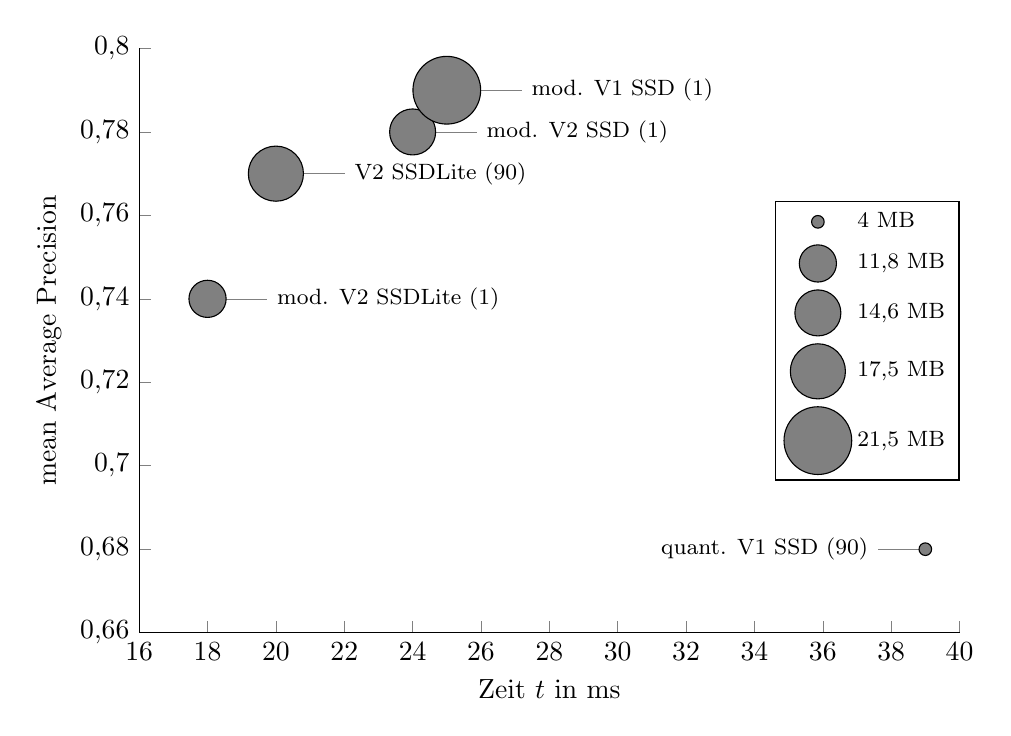
\begin{tikzpicture}
	\begin{axis}[
width=12cm,
height=9cm,
axis y line*=left,
ticklabel style={% gilt für x und y
	/pgf/number format/.cd,
	use comma,% Komma als Dezimaltrenner
	1000 sep = {}% keine Tausendertrennung 
},
xlabel={Zeit $t$ in ms},
ylabel={mean Average Precision},
axis x line*=bottom,
xmin=16, xmax=40, 
ymin=0.66, ymax=0.8,
%every axis plot/.append style={line width=1.0pt}
%legend pos=north east,
legend cell align={left},
legend style={row sep = 0.1cm,at={(1,0.5)},anchor=east} ,
]
\addlegendentry{\footnotesize 4 MB};
\addlegendentry{\footnotesize 11,8 MB};
\addlegendentry{\footnotesize 14,6 MB};
\addlegendentry{\footnotesize 17,5 MB};
\addlegendentry{\footnotesize 21,5 MB};
\addplot[only marks, mark options = {draw =black, scale = 0.04cm, fill = gray}] coordinates{(39,0.68)} node[xshift=0.1cm,pos=0,pin={[pin distance=0.58cm]left:{\footnotesize quant. V1 SSD (90)}}]{} ;
\addplot[only marks, mark options = {draw =black, scale = 0.118cm, fill = gray}] coordinates{(18,0.74)} node[xshift=-0.1cm,pos=0, pin={[pin distance=0.736cm]right:{\footnotesize mod. V2 SSDLite (1)}}]{} ;
\addplot[only marks, mark options = {draw =black, scale = 0.146cm, fill = gray}] coordinates{(24,0.78)} node[xshift=-0.1cm,pos=0, pin={[pin distance=0.792cm]right:{\footnotesize mod. V2 SSD (1)}}]{} ;
\addplot[only marks, mark options = {draw =black, scale = 0.175cm, fill = gray}] coordinates{(20,0.77)} node[xshift=-0.1cm,pos=0, pin={[pin distance=0.85cm]right:{\footnotesize  V2 SSDLite (90)}}]{} ;

\addplot[only marks, mark options = {draw =black, scale = 0.215cm, fill = gray}] coordinates{(25,0.79)} node[xshift=-0.1cm,pos=0, pin={[pin distance=0.93cm]right:{\footnotesize mod. V1 SSD (1)}}]{} ;
\end{axis}
\end{tikzpicture}
	\caption{Vergleich aller untersuchten \textit{MobileNet} Architekturen. Das Diagramm stellt die \textit{mean Average Precision} aufgetragen über die gemessene Rechenzeit dar. Gezeigt ist der Test auf dem integrierten Rechner des ALFs in Anwendung auf den eigenen Datensatz.   }
\label{fig: komplettvergleich}


\end{figure}

